\section{Thiết kế trục I}
\subsection{Chọn vật liệu}
Chọn vật liệu chế tạo là thép $C_{45}$, giới hạn bền $\sigma_b =736MPa$, giới hạn chảy $\sigma_{ch} = 490MPa$.
Ứng suất uốn cho phép $[\sigma_F] = 48MPa$, ứng suất tiếp cho phép $[\tau] = 22MPa$.
\subsection{Phân tích lực trên trục}
\begin{itemize}
    \item Lực tác dụng lên trục của bộ truyền đai: $F_r = 833,8N$
    \item Lực vòng bánh dẫn: $F_{t1} = 2.10^3\frac{T_1}{d_1} = 2.10^3.\frac{63,73}{54,738} = 2328,55N$
    \item Lực hướng tâm trên bánh dẫn: $F_{r1} = \frac{F_{t1}.\tan\alpha}{\cos\beta} = \frac{2328,55.\tan20}{\cos18,2} = 892,1544N$
    \item Lực dọc trục trên banh dẫn: $F_{a1} = F_{t1}.\tan\beta = 2328,55.\tan18,2 = 765,588N$
\end{itemize}

\subsection{Thiết kế sơ bộ kết cấu trục}
Tính sơ bộ đường kính trục: \\
\[
    d_1 = 10\sqrt[3]{\frac{16T_1}{\pi[\tau]}} = 10\sqrt[3]{\frac{16.63,73}{\pi.22}} = 24,526(mm)
\]
$\Rightarrow$ Chọn d = 25mm theo tiêu chuẩn. \\
Khoảng cách giữa các ổ trong hộp giảm tốc bánh răng trụ một cấp: \\
\[
    l \approx l_1 + 2x + w = 85 + 2.10 + 35 = 140(mm)
\]
Trong đó: 
\begin{itemize}
    \item $l_1 = b_1 = 85(mm)$ - Kết quả tính bộ truyền bánh răng
    \item $w = 35(mm) - w = 30 \div 55(mm)$ khi $T = 60 \div 80(Nm)$
    \item $x = 10(mm)$ - Khe hở giữa bánh răng và thành trong hộp giảm tốc
\end{itemize}
Khoảng cách f theo bảng 10.3 không nhỏ hơn $55 \div 75$ nên ta chọn $f = 60mm.$
\subsection{Vẽ biểu đồ momen uốn và xoắn}
Trong mặt phẳng đứng zy, phương trình cân bằng momen: $M_{A} = 0$ \\
Suy ra:
\[
    F_r .0,06 - F_{r1}.0,07 + M_{a1} + R_{BY}.0,14 = 0
\]
Trong đó $M_{a1} = \frac{F_{a1}.d_1.10^{-3}}{2} = \frac{765,588.54,738.10^{-3}}{2} = 20,95Nm$ \\
\begin{equation}
    \Leftrightarrow 833,8.0,06 - 892,1544.0,07 + 20,95 + R_{BY}.0,14 = 0
\end{equation}
Phương trình cân bằng lực theo trục y: \\
\[
    -F_r + R_{AY} + -F_{r1} + R_{BY} = 0
\]
\begin{equation}
    \Leftrightarrow -833,8 + R_{AY} - 892,1544 + R_{BY} = 0
\end{equation}
Từ (1) và (2) ta giải hệ phương trình tìm được $R_{AY} = 1786,86N$ và $R_{BY} = -60,9N$. \\
Trong mặt phẳng nằm ngang zx, vì lực $F_{t1}$ nằm đối xứng với hai ổ, nên: 
\[
    R_{AX} = R_{BX} = \frac{F_{t1}}{2} = \frac{2328,55}{2} = 1164,27N
\]
Vẽ biểu đồ momen với:
\begin{itemize}
    \item $M_{XD} = R_{BY}.0,07 = 4,263Nm$
    \item $M_{XA} = F_r.0,06 = 50,028Nm$
    \item $M_{YD} = R_{BX}.0,07 = 81,5Nm$
\end{itemize}   
Momen xoắn T1 = 63,73Nm. \\
\begin{figure}[H]
    \centering
    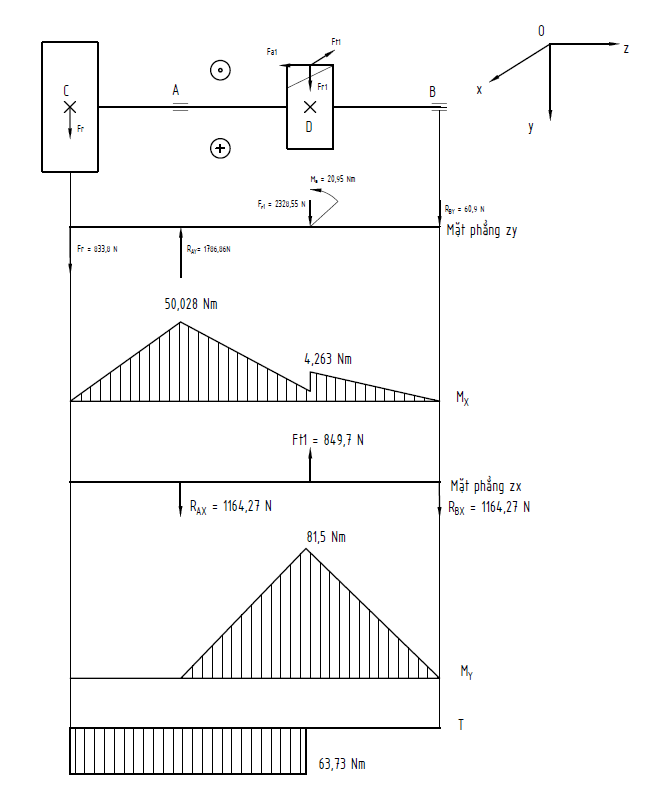
\includegraphics[width=1.1\textwidth]{pictures/luctruc1.png}
\end{figure}
\subsection{Momen uốn và momen xoắn tại vị trí nguy hiểm}
Các biểu đồ momen cho thấy tiết diện nguy hiểm nhất tại vị trí D. \\
Momen uốn tại D: 
\[
    M_D = \sqrt{M_{XD}^2 + M_{YD}^2} = \sqrt{4,263^2 + 81,5^2} = 81,61Nm
\]
Momen xoắn tại D: $T = 63,73Nm$ \\
Momen tương đương tại D: \\
$M_{td} = \sqrt{M_{XD}^2 + M_{YD}^2 + 0,75T^2} = \sqrt{4,263^2 + 81,5^2 + 0,75.63,73^2} = 98,52 Nm$\\
\[
d = \sqrt[3]{\frac{M_{td}.10^3}{0,1.[\sigma]}} = 27,38 mm
\]
Tại vị trí D có lắp bánh răng nên cần tăng đường kính trục thêm 5\% nên chọn d = 30mm. 
\subsection{Ứng suất pháp tại tiết diện D}
Ta bỏ qua ảnh hưởng của lực dọc trục nên ứng suất pháp tại tiết diện này thay đổi theo
chu kỳ đối xứng biên độ:
\[  
    \sigma_a = \sigma_F = \frac{M_D.10^3}{W}
\]
Tại vị trí D trục có một then, với đường kính d = 30mm, ta chọn then có chiều rộng $b = 8mm$, chiều cao $h = 7mm$, chiều sâu rãnh then trên trục t = 4mm, chiều sâu rãnh then trên mayơ $t_1 = 3,8 mm$. Khi đó: 
\[
    W = \frac{\pi d^3}{32} - \frac{bt(d-t)^2}{2d} = \frac{\pi 25^3}{32} - \frac{8.4(25-4)^2}{2.25} = 1251,741mm^3
\]
Do đó:  
\[
    \sigma_a = \frac{98,52.10^3}{1251,741} = 78,706MPa
\]
\begin{figure}[H]
    \centering
    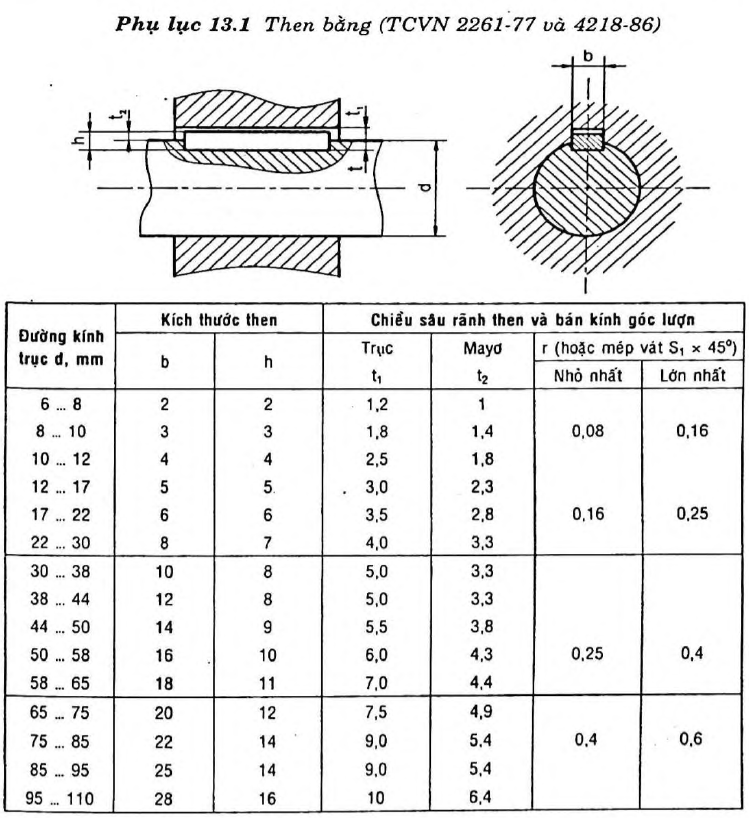
\includegraphics[width=0.8\textwidth]{pictures/then.png}
    \caption{Tiêu chuẩn chọn then}
\end{figure}
\subsection{Kiểm nghiệm then tại vị trí gắn bánh răng D}
\begin{figure}[H]
    \centering
    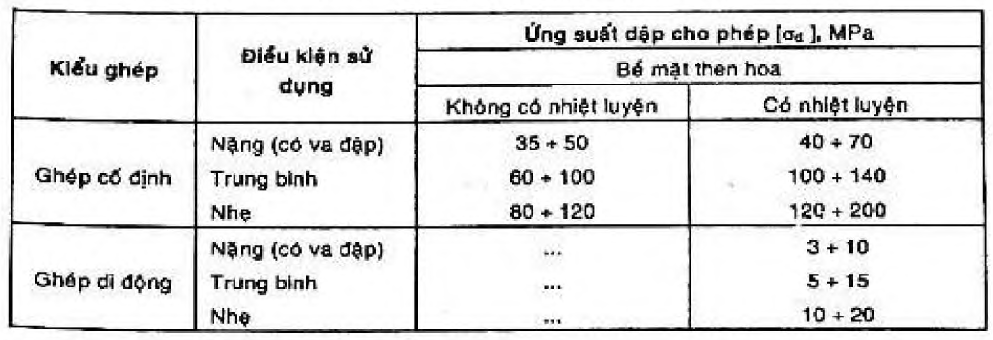
\includegraphics[width=0.8\textwidth]{pictures/then1.png}
    \caption{Trị số ứng xuất dập cho phép của then hoa}
\end{figure}
Chọn chiều dài l của then theo tiêu chuẩn l = 56mm.\\
Chọn ứng suất dập cho phép $[\sigma_d]$ = 150MPa theo bảng 16.1. \\
Chọn ứng suất cắt cho phép $[\tau_d]$ = 90MPa \\
Kiểm tra độ bền dập theo công thức:
\[
    \sigma_d = \frac{F}{t_2l_l} = \frac{2T.10^3}{t_2dl_l} = \frac{2.63,73.10^3}{2,8.25.48} = 37,9MPa < [\sigma_d] = 150MPa
\]
Trong đó:
\begin{itemize}
    \item $l_l = l - b = 56 - 8 = 48mm$
    \item $h = 7mm$
    \item $t_2 = 0,4h = 2,8mm$
\end{itemize}
Kiểm tra then theo độ bền cắt: 
\[
    \tau_d = \frac{T}{bl_l} = \frac{2T.10^3}{bdl_l} = \frac{2.63,73.10^3}{8.25.48} = 13,28MPa < [\tau_d] = 90MPa 
\]
$\Rightarrow$ Vậy then này đạt độ bền tính toán.
\subsection{Ứng suất xoắn tại vị trí D}
\[
    \tau = \frac{T_1.10^3}{W_o} = \frac{63,73.10^3}{2785,7216} = 22,88MPa
\]
Trong đó momen cản xoắn:
\[
    W_o = \frac{\pi d^3}{16} - \frac{bt(d-t)^2}{2d} = \frac{\pi 25^3}{16} - \frac{8.4(25-4)^2}{2.25} = 2785,7216mm^3
\]
Khi ứng suất xoắn thay đổi theo chu kỳ mạch động: 
\[
    \tau_\alpha = \sigma_m = \frac{\sigma}{2} = \frac{22,88}{2} = 11,44MPa
\]
\subsection{Xác định hệ số an toàn tại vị trí D}
Tại tiết diện D có sự tập trung ứng suất là rãnh then. Theo bảng 10.9 ta chọn $K_\sigma =2,05$, $K_\tau = 1,9$ với $\sigma_b = 736MPa < 800MPa$ \\
Theo bảng 10.4 với d = 30mm ta chọn $\epsilon_\sigma = 0,91$ và $\epsilon_\tau = 0.89$ \\
Hệ số $\Psi_\sigma = 0,035$ và $\Psi_\tau = 0,07$ \\ 
Với hệ số tăng bền bề mặt, chọn phương pháp phun bi nên $\beta = 1,7$. \\
Với thép C45, d =25mm chọn giới hạn mỏi của vật liệu $\sigma_{-1} = 432MPa$, $\tau_{-1} = 255MPa$. \\
Xác định hệ số an toàn tại D theo công thức:
\[
    s_\sigma = \frac{\sigma_{-1}}{K_\sigma \sigma_a / \epsilon_\sigma \beta + \Psi_\sigma \sigma_m} = \frac{432}{2,05.66,47/0,91.1,7 + 0,035.0} = 4,9
\]
\[
    s_\tau = \frac{\tau_{-1}}{K_\tau \tau_a / \epsilon_\tau \beta + \Psi_\tau \tau_m} = \frac{255}{2,05.11,44/0,89.1,7 + 0,07.11,44} = 15,943
\]
Hệ số an toàn:
\[
    s = \frac{s_\sigma s_\tau}{\sqrt{s_\sigma^2 + s_\tau^2}} = \frac{4,9.15,943}{\sqrt{4,9^2 + 15,943^2}} = 4,684 > [s] = 1,5
\]
Do đó điều kiện bền mỏi của trục tại tiết diện D được thỏa.
\subsection{Ứng suất pháp tại tiết diện C}
Ta bỏ qua ảnh hưởng của lực dọc trục nên ứng suất pháp tại tiết diện này thay đổi theo chu kỳ đối xứng biên độ:
\[
    \sigma_a = \sigma_F = \frac{M_C.10^3}{W}
\]
Trong đó $M_C = \sqrt{M_{CX}^2 + M_{CY}^2 + 0,75T^2} = 55,19 Nm$\\
Tại vị trí C trục có một then, với đường kính d = 30mm, ta chọn then có chiều rộng $b = 8mm$, chiều cao $h = 7mm$, chiều sâu rãnh then trên trục t = 4mm, chiều sâu rãnh then trên mayơ $t_1 = 3,8 mm$. Khi đó: 
\[
    W = \frac{\pi d^3}{32} - \frac{bt(d-t)^2}{2d} = \frac{\pi 25^3}{32} - \frac{8.4(25-4)^2}{2.25} = 1251,741mm^3
\]
Do đó:  
\[
    \sigma_a = \frac{55,19.10^3}{1251,741} = 44,09MPa
\]
\subsection{Kiểm nghiệm then tại vị trí gắn bánh đai C}
Chọn chiều dài l của then theo tiêu chuẩn l = 56mm.\\
Chọn ứng suất dập cho phép $[\sigma_d]$ = 150MPa theo bảng 16.1. \\
Chọn ứng suất cắt cho phép $[\tau_d]$ = 90MPa \\
Kiểm tra độ bền dập theo công thức:
\[
    \sigma_d = \frac{F}{t_2l_l} = \frac{2T.10^3}{t_2dl_l} = \frac{2.63,73.10^3}{2,8.25.48} = 37,9MPa < [\sigma_d] = 150MPa
\]
Trong đó:
\begin{itemize}
    \item $l_l = l - b = 56 - 8 = 48mm$
    \item $h = 7mm$
    \item $t_2 = 0,4h = 2,8mm$
\end{itemize}
Kiểm tra then theo độ bền cắt: 
\[
    \tau_d = \frac{T}{bl_l} = \frac{2T.10^3}{bdl_l} = \frac{2.63,73.10^3}{8.25.48} = 13,28MPa < [\tau_d] = 90MPa 
\]
$\Rightarrow$ Vậy then này đạt độ bền tính toán.
\subsection{Ứng suất xoắn tại vị trí C}
\[
    \tau = \frac{T_1.10^3}{W_o} = \frac{63,73.10^3}{2785,7216} = 22,88MPa
\]
Trong đó momen cản xoắn:
\[
    W_o = \frac{\pi d^3}{16} - \frac{bt(d-t)^2}{2d} = \frac{\pi 25^3}{16} - \frac{8.4(25-4)^2}{2.25} = 2785,7216mm^3
\]
Khi ứng suất xoắn thay đổi theo chu kỳ mạch động: 
\[
    \tau_\alpha = \sigma_m = \frac{\sigma}{2} = \frac{22,88}{2} = 11,44MPa
\]
\subsection{Xác định hệ số an toàn tại vị trí C}
Tại tiết diện D có sự tập trung ứng suất là rãnh then. Theo bảng 10.9 ta chọn $K_\sigma =2,05$, $K_\tau = 1,9$ với $\sigma_b = 736MPa < 800MPa$ \\
Theo bảng 10.4 với d = 30mm ta chọn $\epsilon_\sigma = 0,91$ và $\epsilon_\tau = 0.89$ \\
Hệ số $\Psi_\sigma = 0,035$ và $\Psi_\tau = 0,07$ \\ 
Với hệ số tăng bền bề mặt, chọn phương pháp phun bi nên $\beta = 1,7$. \\
Với thép C45, d =30mm chọn giới hạn mỏi của vật liệu $\sigma_{-1} = 432MPa$, $\tau_{-1} = 255MPa$. \\
Xác định hệ số an toàn tại D theo công thức:
\[
    s_\sigma = \frac{\sigma_{-1}}{K_\sigma \sigma_a / \epsilon_\sigma \beta + \Psi_\sigma \sigma_m} = \frac{432}{2,05.40,09/0,91.1,7 + 0,035.0} = 8,13
\]
\[
    s_\tau = \frac{\tau_{-1}}{K_\tau \tau_a / \epsilon_\tau \beta + \Psi_\tau \tau_m} = \frac{255}{2,05.11,44/0,89.1,7 + 0,07.11,44} = 15,943
\]
Hệ số an toàn:
\[
    s = \frac{s_\sigma s_\tau}{\sqrt{s_\sigma^2 + s_\tau^2}} = \frac{8,13.15,943}{\sqrt{8,13^2 + 15,943^2}} = 7,24 > [s] = 1,5
\]
Do đó điều kiện bền mỏi của trục tại tiết diện C được thỏa.